\documentclass{beamer}

\mode<presentation> {

% The Beamer class comes with a number of default slide themes
% which change the colors and layouts of slides. Below this is a list
% of all the themes, uncomment each in turn to see what they look like.
\usepackage{mdframed}
%\usetheme{default}
%\usetheme{AnnArbor}
%\usetheme{Antibes}
%\usetheme{Bergen}
%\usetheme{Berkeley}
\usetheme{Berlin}
%\usetheme{Boadilla}
%\usetheme{CambridgeUS}
%\usetheme{Copenhagen}
%\usetheme{Darmstadt}
%\usetheme{Dresden}
%\usetheme{Frankfurt}
%\usetheme{Goettingen}
%\usetheme{Hannover}
%\usetheme{Ilmenau}
%\usetheme{JuanLesPins}
%\usetheme{Luebeck}
%\usetheme{Madrid}
%\usetheme{Malmoe}
%\usetheme{Marburg}
%\usetheme{Montpellier}
%\usetheme{PaloAlto}
%\usetheme{Pittsburgh}
%\usetheme{Rochester}
%\usetheme{Singapore}
%\usetheme{Szeged}
%\usetheme{Warsaw}

% As well as themes, the Beamer class has a number of color themes
% for any slide theme. Uncomment each of these in turn to see how it
% changes the colors of your current slide theme.

%\usecolortheme{albatross}
%\usecolortheme{beaver}
%\usecolortheme{beetle}
%\usecolortheme{crane}
%\usecolortheme{dolphin}
%\usecolortheme{dove}
%\usecolortheme{fly}
%\usecolortheme{lily}
%\usecolortheme{orchid}
%\usecolortheme{rose}
%\usecolortheme{seagull}
%\usecolortheme{seahorse}
%\usecolortheme{whale}
%\usecolortheme{wolverine}

%\setbeamertemplate{footline} % To remove the footer line in all slides uncomment this line
%\setbeamertemplate{footline}[page number] % To replace the footer line in all slides with a simple slide count uncomment this line

%\setbeamertemplate{navigation symbols}{} % To remove the navigation symbols from the bottom of all slides uncomment this line
}

\usepackage{graphicx} % Allows including images
\usepackage{booktabs} % Allows the use of \toprule, \midrule and \bottomrule in tables

%----------------------------------------------------------------------------------------
%	TITLE PAGE
%----------------------------------------------------------------------------------------

\title[Short title]{Web Scraping with Scrapy} % The short title appears at the bottom of every slide, the full title is only on the title page

\author{Akshay Krishna} % Your name
\institute[] % Your institution as it will appear on the bottom of every slide, may be shorthand to save space
{
S5 CSE A \\ % Your institution for the title page
\medskip
\textit{} % Your email address
}
\date{\today} % Date, can be changed to a custom date

\begin{document}

\begin{frame}
\titlepage % Print the title page as the first slide
\end{frame}

\begin{frame}
\frametitle{Objective}
\begin{itemize}
\item \textbf {Scrap information from webpages of a given website using Scrapy}
\end{itemize}
\end{frame}

\begin{frame}
\frametitle{What is Web scraping ? What is it's relevence ?}
Web scraping refers to the process of collecting and organizing data from a web page. Today various methods are used to scrape data from web pages. The process of web scraping mainly involves two steps.Fetching and Extracting. First the agent requests the web page. When the web page is fetched as aknowledgement for the request,in the next step we extracts the required information from the fetched web page.
\\
Web scraping nowadays used for purposes like, contact scraping,and as a component of webapplications used for web indexing,web mining and data mining,price comparison,weather data monitoring,researching etc.
\end{frame}

\begin{frame}
\frametitle{Existing methods}
\begin{block}{1.Human Copy-Paste}
A human being manuals examines the webpage and copy paste required data. Failure rate is almost zero in this traditional technique
\end{block}
\begin{block}{2.Text pattern matching}
An approach to extract information from webpage using UNIX \textbf{grep} command or regular expression matching facilities of programming languages
\end{block}
\end{frame}

\begin{frame}
\begin{block}{3.Using web-scraping framewors/softwares}
These frameworks/softwares gives the facilities to create web scraping bots(spiders/crawlers) to scrape data from webpages.These spiders try to recognize structure of the page automaticaly and extracts the data and gives the facility to process and store them in specific format
\end{block}

\begin{block}{4.Computer vision webpage analysis}
Employing the features of machine learning and computer vision to idenetify and extract data from webpage. This can be described as computerised version of human copy-paste with a failure rate >0
\end{block}
\end{frame}

\begin{frame}[fragile]
\frametitle{Proposed Methodology}
\textbf{Using web-scraping framework}
\\*
The proposed methodology is to scrape webpages using a software/framework. Here we are using "Scrapy", a framework written in python to generate and deploy spiders to extract data from a webpage
\begin{mdframed}
\textbf{Why Scrapy ?}
\begin{enumerate}
\item Faster and automated way to scrape webpages
\item Easy to use \& implement
\item Have selectors to specify data field needs to be extracted
\item Have pipelines to refine extracted data
\end{enumerate}
\end{mdframed}
\end{frame}

\begin{frame}
\frametitle{ How Scrapy works}
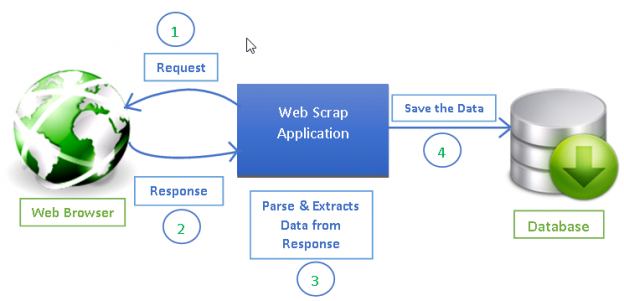
\includegraphics[scale=.5]{custom-web-scraping-624x301.png} 
\end{frame}

\begin{frame}{Barriers to Web Scraping}
\begin{itemize}
\item Not all web pages allows data scraping
\item Captchas block the scraper from proceding further
\item Frequent structural changes made to website
\item IP blocking
\end{itemize}
\end{frame}

\begin{frame}
\frametitle{Implementation Algorithm}
\center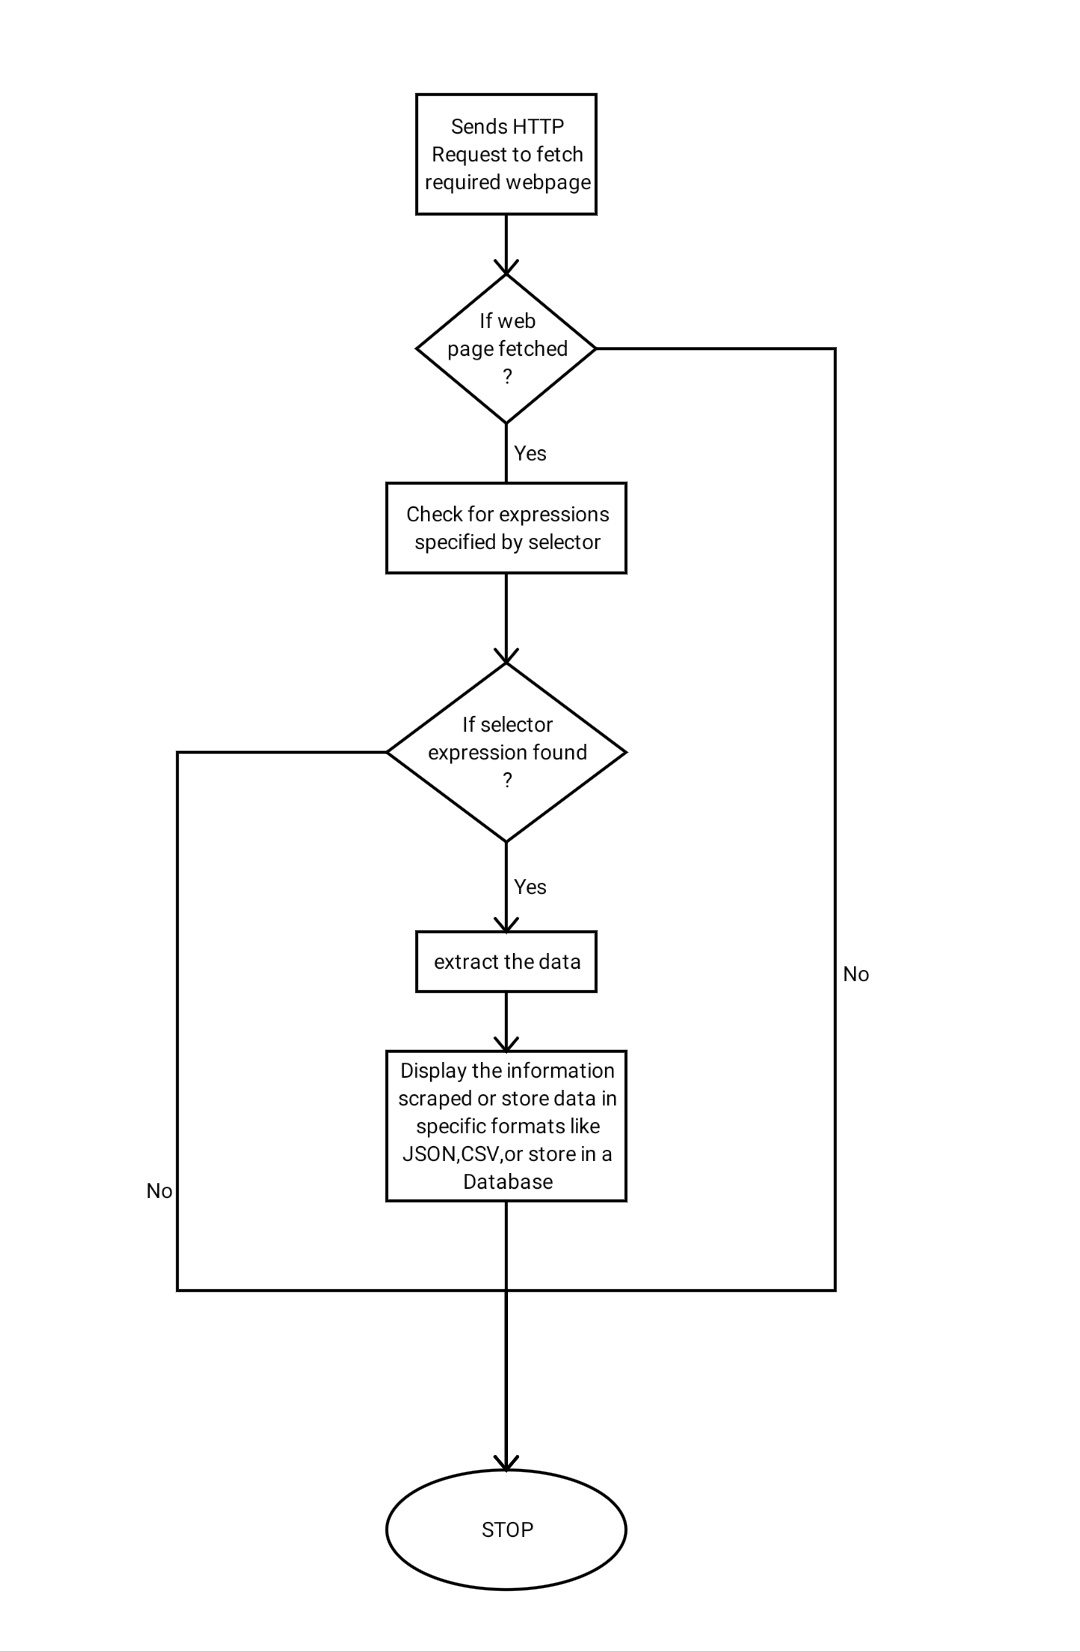
\includegraphics[scale=.12]{IMG_20191017_083215.jpg} 
\end{frame}

\begin{frame}
\frametitle{Conclusion}

Webpages of given Website is scraped and extracted data displayed in a specific format
\end{frame}
\end{document}